% !TeX program = xelatex
% ============================================================
% 1989 年·广东卷文科候选卷 · 试题版
% 由 tools/make_editions.py 生成（重跑会覆盖本文件）；
% 题目/解析内容在 questions.tex / answers*.tex，勿在本文件内写内容。
% ============================================================
\documentclass[zihao=-4, a4paper]{ctexart}
% ============================================================
% common/preamble.tex —— 拆分版试卷项目 · 公共导言区
% 引擎：XeLaTeX；文档类 ctexart 由各版本壳文件自行声明
% 由合并书 math-gaokao-2017-2026/preamble.tex 改造而来：
%   - 页眉左右改为可重定义宏 \gkheadL / \gkheadR（各版本壳设置）
%   - hyperref 不再写死 pdftitle（壳内 \hypersetup 覆盖）
%   - 删除书籍专用的 \chaptermark 重定义与 \gkpaper 装配宏
% ============================================================

% ---------- 数学 ----------
\usepackage{amsmath}
\usepackage{amssymb}
\usepackage{mathtools}

% ---------- 绘图 ----------
\usepackage{tikz}
\usetikzlibrary{shapes.geometric, arrows.meta, calc, patterns, angles, quotes, positioning}
\usepackage{pgfplots}
\pgfplotsset{compat=1.18}

% ---------- 版面 ----------
\usepackage{geometry}
\usepackage{needspace}
\geometry{a4paper, margin=2.2cm, headheight=15pt}
% 紧凑版式（如印刷版）可在壳文件中于 \begin{document} 前再次调用 \geometry 覆盖
\usepackage{enumitem}
\setlist{itemsep=2pt, topsep=4pt, parsep=0pt}

% 中文与行内公式混排的断行弹性：
% emergencystretch 允许段落末路不通时追加伸展量；
% 降低二元/关系符罚分，允许行内长公式在 = 、+ 等处断行（否则整段外溢）
\emergencystretch=2em
\binoppenalty=700
\relpenalty=500
\usepackage{booktabs}      % 三线表
\usepackage[most]{tcolorbox}

% ---------- 选择题选项对齐 ----------
% tasks 宏包：\begin{gkopts}(列数) \task ... \end{gkopts}
% 自动等宽分栏，选项天然对齐；列数已由内容片段按选项长度写定（4/2/1）
\usepackage{tasks}
\settasks{label={}, label-width=0pt, item-indent=1.2em,
          column-sep=1em, after-item-skip=2pt, before-skip=2pt, after-skip=4pt}
\NewTasksEnvironment[style=itemize]{gkopts}[\task](4)

% ---------- 页眉页脚 ----------
\newcommand{\gkheadL}{}   % 左页眉：卷名（壳文件 \renewcommand 设置）
\newcommand{\gkheadR}{}   % 右页眉：版本名（壳文件 \renewcommand 设置）
\usepackage{fancyhdr}
\pagestyle{fancy}
\fancyhf{}
\fancyhead[L]{\small\gkheadL}
\fancyhead[R]{\small\gkheadR}
\fancyfoot[C]{\small —— 第 \thepage\ 页 ——}
\renewcommand{\headrulewidth}{0.4pt}

% ---------- 超链接（须最后加载）----------
\usepackage{hyperref}
\hypersetup{colorlinks=true, linkcolor=blue!55!black,
            bookmarksnumbered=true, unicode=true}

% ============================================================
% common/macros.tex —— 自定义命令与环境（题号、解析头、提示框等）
% 与合并书 math-gaokao-2017-2026/preamble.tex 的自定义段保持一致，
% 保证内容片段（questions.tex / answers.tex）在两个项目间可互换。
% ============================================================

% ---------- 试卷标识（壳文件 \renewcommand 设置，用于 label 命名空间）----------
\newcommand{\gkpaperid}{none}

% ---------- 题号 ----------
% 试题部分的题号：加粗编号 + 自动 \label{q:<卷id>:<题号>}
\newcommand{\gkti}[1]{\par\medskip\noindent
  \textbf{#1．}\phantomsection\label{q:\gkpaperid:#1}\ignorespaces}
% 多卷/分部重启题号时，#1 是唯一内部顺序号（交叉引用身份），#2 才是原卷显示题号。
\newcommand{\gktiwithlabel}[2]{\par\medskip\noindent
  \textbf{#2．}\phantomsection\label{q:\gkpaperid:#1}\ignorespaces}

% 解析部分的题头：小标题 + 回链到试题页
% （仅在题目与解析同文档的版本中回链有效；试题版不含解析头，无悬空引用）
\newcommand{\gksolhead}[2]{%
  \Needspace{3\baselineskip}\subsubsection*{第 #1 题\if\relax\detokenize{#2}\relax\else（#2）\fi}%
  \phantomsection\label{s:\gkpaperid:#1}%
  {\small\color{gray}（题目见第~\pageref{q:\gkpaperid:#1}~页）}\par\nopagebreak}
% 与 \gktiwithlabel 成对：显示原题号，但回链仍用唯一内部顺序号。
\newcommand{\gksolheadwithlabel}[3]{%
  \Needspace{3\baselineskip}\subsubsection*{第 #2 题\if\relax\detokenize{#3}\relax\else（#3）\fi}%
  \phantomsection\label{s:\gkpaperid:#1}%
  {\small\color{gray}（题目见第~\pageref{q:\gkpaperid:#1}~页）}\par\nopagebreak}

% ---------- 填空题空位 ----------
\newcommand{\gkblank}{\underline{\hspace{2.2em}}}

% ---------- 提示框 ----------
% 卷种提示 / 解析归属声明（醒目，浅黄）
\newtcolorbox{gknotice}{colback=yellow!8, colframe=orange!60!black,
  boxrule=0.5pt, arc=1.5pt, left=6pt, right=6pt, top=4pt, bottom=4pt,
  before skip=8pt, after skip=8pt}

% 方法提示 / 注（浅蓝，用于解析后的点评与题量说明）
\newtcolorbox{gktip}{colback=blue!4, colframe=blue!35!black,
  boxrule=0.4pt, arc=1.5pt, left=6pt, right=6pt, top=4pt, bottom=4pt,
  before skip=6pt, after skip=6pt, fontupper=\small}

% ---------- 答案行 ----------
% 解析中独立成段的"答案：X"用带底色的行呈现
\newcommand{\gkanswer}[1]{\par\smallskip\noindent
  \tcbox[width=\linewidth, tcbox width=auto limited,
         colback=green!6, colframe=green!35!black, boxrule=0.4pt,
         arc=1.5pt, left=4pt, right=4pt, top=2pt, bottom=2pt,
         nobeforeafter]{\textbf{#1}}\par\smallskip}

% ---------- 结构标题 ----------
% 结构标题后通常紧跟一个带 0.5\textheight 起始预留的解析题块；0.4 只够放标题，
% 会把下一题整体推到下一页，留下孤立的「二、填空题」等页尾标题。
\newcommand{\gkpart}[1]{\Needspace{0.6\textheight}\subsection*{#1}\nopagebreak}     % 标题 + 首题
% （一）必考题 / 解析小问标题：块式加粗段，可自动换行（\paragraph 的 run-in 版式会溢出）
\newcommand{\gksubpart}[1]{\Needspace{6\baselineskip}\par\medskip\noindent\textbf{#1}\par\nopagebreak\smallskip}

% 罗马数字Ⅰ-Ⅻ（U+2160）与圈号①②③（U+2460）划入 CJK 字符类，
% 用中文字体渲染——西文字体 Latin Modern 缺这些字形，否则整段静默丢字
\xeCJKDeclareCharClass{CJK}{"2160 -> "217F, "2460 -> "24FF}

% ============================================================
% common/questions_env.tex —— 题目 / 解析的语义包装环境
%
% questions.tex 中每道题包在 \begin{question}...\end{question} 里，
% answers.tex 中每题解析包在 \begin{answer}...\end{answer} 里；
% 题头排版仍由内容行中的 \gkti / \gksolhead 完成（见 macros.tex）。
%
% 环境本身不产生任何盒子或垂直间距（只引入一个 TeX 分组），
% 排版结果与不包裹时逐点一致。它的价值在于：
%   1. 给每道题一个机器可数的结构边界（校验脚本数环境数 = 题量）；
%   2. 为将来的条件编译留钩子——某版本可重定义环境实现按题取舍。
% ============================================================

% 环境不把整题装盒：题目与解析仍可自然跨页，但开始题块前必须为题面、
% 图形/表格或解析首段留出足够空间。仅保留 2 个 baseline 会让题干、
% 选项和图形在页边界处被拆开，形成不可打印的孤立内容；题目保留
% 0.15\textheight，在避免短题制造大段空白与避免题块拆分之间取平衡。
% 解析题块保留 0.5\textheight，以容纳“题面 + 图形/选项 + 首段解析”；
% 结构标题仍用更大的保留量；末页自然收尾由视觉复审判定。
\newenvironment{question}{\Needspace{0.15\textheight}}{}
\newenvironment{answer}{\Needspace{0.5\textheight}}{}

\renewcommand{\gkpaperid}{gk-1989-regular-guangdong-arts}
\renewcommand{\gkheadL}{1989 年·广东卷文科候选卷 · 数学}
\renewcommand{\gkheadR}{试题版}
\hypersetup{pdftitle={1989 年·广东卷文科候选卷 数学 · 试题版}}
\begin{document}
\begin{center}
  {\Large\bfseries 1989 年·广东卷文科候选卷}\\[4pt]
  {\large 数学 · 试题版}
\end{center}
\medskip
\pdfbookmark[1]{试题}{sec:q}
% questions.tex —— 1989 年·广东卷文科候选卷 · 题目内容片段（无答案）
% 由 tools/generate_projects.py 依来源总账自 1989/1989_数学真题_广东文_试题.md 生成，勿手改（改源 MD 后重跑）


\begin{gktip}
固定来源扫描件题签仅见“文史类”，未印年份或出版者标识；1989 年份及广东卷归属依据仓库固定来源记录。以下只转录该固定文件可见题面，不据第三方记忆补字。原件为9页扫描，扫描页1—7为题面，页8—9为答案及解析；图形用矢量示意源重绘，不以扫描截图代替。
\end{gktip}

\gkpart{第一卷：选择题（25题，共50分）}

每题给出 A、B、C、D 四个结论，其中只有一个结论正确。每题选对得2分，不选、选错或选出的代号超过一个，一律得0分。

\begin{question}
\gkti{1}函数 $f(x)=x^{1/5}$（　）。

\begin{gkopts}(2)
\task A．是奇函数而不是偶函数；
\task B．是偶函数而不是奇函数；
\task C．既是奇函数又是偶函数；
\task D．既不是奇函数又不是偶函数。
\end{gkopts}

\end{question}
\begin{question}
\gkti{2}函数 $y=\lg x\ (x>0)$ 的值域是（　）。

\begin{gkopts}(2)
\task A．$(0,+\infty)$；
\task B．$(-\infty,0)$；
\task C．$(-\infty,+\infty)$；
\task D．$[0,+\infty)$。
\end{gkopts}

\end{question}
\begin{question}
\gkti{3}直线 $x+\sqrt3y-3=0$ 的倾斜角是（　）。

\begin{gkopts}(4)
\task A．$\dfrac\pi6$；
\task B．$\dfrac\pi3$；
\task C．$\dfrac23\pi$；
\task D．$\dfrac56\pi$。
\end{gkopts}

\end{question}
\begin{question}
\gkti{4}二面角是指（　）。

\begin{gkopts}(2)
\task A．两个平面所组成的角；
\task B．经过同一直线的两个平面所组成的图形；
\task C．从一条直线出发的两个半平面所组成的图形；
\task D．两个平面所夹的不大于 $90^\circ$ 的角。
\end{gkopts}

\end{question}
\begin{question}
\gkti{5}对数方程 $2\log_x 8-3\log_8 x=1$ 的解集是（　）。

\begin{gkopts}(2)
\task A．$\{4,\tfrac18\}$；
\task B．$\{2,\tfrac{\sqrt2}{4}\}$；
\task C．$\{4,\tfrac14\}$；
\task D．$\{2,\tfrac18\}$。
\end{gkopts}

\end{question}
\begin{question}
\gkti{6}如果 $\sin(\pi+A)=-\dfrac12$，那么 $\cos\left(\dfrac{3\pi}2-A\right)=$（　）。

\begin{gkopts}(2)
\task A．$\dfrac12$；
\task B．$-\dfrac12$；
\task C．$\dfrac{\sqrt3}2$；
\task D．$-\dfrac{\sqrt3}2$。
\end{gkopts}

\end{question}
\begin{question}
\gkti{7}平移坐标轴，把原点移到 $O'(3,-4)$，那么点 $(3,-2)$ 的新坐标是（　）。

\begin{gkopts}(4)
\task A．$(6,-6)$；
\task B．$(-3,4)$；
\task C．$(0,-2)$；
\task D．$(0,2)$。
\end{gkopts}

\end{question}
\begin{question}
\gkti{8}如果直线 $l$ 与直线 $y=2x-1$ 关于直线 $y=x$ 对称，那么直线 $l$ 的方程是（　）。

\begin{gkopts}(2)
\task A．$y=2x-1$；
\task B．$y=\dfrac12x+1$；
\task C．$y=\dfrac12x-\dfrac12$；
\task D．$y=\dfrac12x+\dfrac12$。
\end{gkopts}

\end{question}
\begin{question}
\gkti{9}设 $A$ 是直角坐标平面上所有的点组成的集合。如果由 $A$ 到 $A$ 的一一对应映射 $f$，使象集合的元素 $(y-1,x+2)$ 和原象集合的元素 $(x,y)$ 对应，那么象点 $(3,-4)$ 的原象点是（　）。

\begin{gkopts}(4)
\task A．$(-5,5)$；
\task B．$(-6,4)$；
\task C．$(2,-2)$；
\task D．$(4,-6)$。
\end{gkopts}

\end{question}
\begin{question}
\gkti{10}不等式 $(x^2-4x-5)(x^2+8)<0$ 的解集是（　）。

\begin{gkopts}(2)
\task A．$\{x\mid -1<x<5\}$；
\task B．$\{x\mid x<-1\text{ \text{或} }x>5\}$；
\task C．$\{x\mid 0<x<5\}$；
\task D．$\{x\mid -1<x<0\}$。
\end{gkopts}

\end{question}
\begin{question}
\gkti{11}等差数列 $\{a_n\}$ 的首项 $a_1=1$，公差 $d\ne0$。如果 $a_1,a_2,a_5$ 成等比数列，那么 $d=$（　）。

\begin{gkopts}(2)
\task A．$3$；
\task B．$2$；
\task C．$-2$；
\task D．$2$ 或 $-2$。
\end{gkopts}

\Needspace{0.4\textheight}
\end{question}
\begin{question}
\gkti{12}函数 $y=|x-1|$ 的图象是（　）。
\nopagebreak[4]
\begin{center}% 按固定来源第3扫描页四个候选图重绘；保留 x=1 参考线、y=1 虚线及折线相对关系。
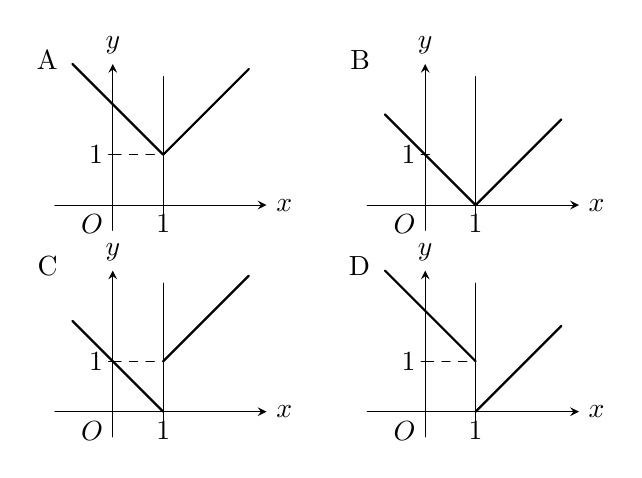
\begin{tikzpicture}[x=0.64cm,y=0.64cm,line cap=round,line join=round,>=stealth]
\begin{scope}
  \draw[->] (-1.15,0)--(3.05,0) node[right] {$x$};
  \draw[->] (0,-0.5)--(0,2.8) node[above] {$y$};
  \draw[thin] (1,-0.35)--(1,2.55);
  \draw[thick] (-0.8,2.8)--(1,1)--(2.7,2.7);
  \draw[dashed] (0,1)--(1,1);
  \draw[thin] (-0.08,1)--(0.08,1) (1,-0.08)--(1,0.08);
  \node[below left] at (0,0) {$O$};
  \node[left] at (0,1) {$1$};
  \node[below] at (1,0) {$1$};
  \node[above left] at (-0.9,2.5) {A};
\end{scope}
\begin{scope}[shift={(6.2,0)}]
  \draw[->] (-1.15,0)--(3.05,0) node[right] {$x$};
  \draw[->] (0,-0.5)--(0,2.8) node[above] {$y$};
  \draw[thin] (1,-0.35)--(1,2.55);
  \draw[thick] (-0.8,1.8)--(1,0)--(2.7,1.7);
  \draw[thin] (-0.08,1)--(0.08,1) (1,-0.08)--(1,0.08);
  \node[below left] at (0,0) {$O$};
  \node[left] at (0,1) {$1$};
  \node[below] at (1,0) {$1$};
  \node[above left] at (-0.9,2.5) {B};
\end{scope}
\begin{scope}[shift={(0,-4.1)}]
  \draw[->] (-1.15,0)--(3.05,0) node[right] {$x$};
  \draw[->] (0,-0.5)--(0,2.8) node[above] {$y$};
  \draw[thin] (1,-0.35)--(1,2.55);
  \draw[thick] (-0.8,1.8)--(1,0);
  \draw[thick] (1,1)--(2.7,2.7);
  \draw[dashed] (0,1)--(1,1);
  \draw[thin] (-0.08,1)--(0.08,1) (1,-0.08)--(1,0.08);
  \node[below left] at (0,0) {$O$};
  \node[left] at (0,1) {$1$};
  \node[below] at (1,0) {$1$};
  \node[above left] at (-0.9,2.5) {C};
\end{scope}
\begin{scope}[shift={(6.2,-4.1)}]
  \draw[->] (-1.15,0)--(3.05,0) node[right] {$x$};
  \draw[->] (0,-0.5)--(0,2.8) node[above] {$y$};
  \draw[thin] (1,-0.35)--(1,2.55);
  \draw[thick] (-0.8,2.8)--(1,1);
  \draw[thick] (1,0)--(2.7,1.7);
  \draw[dashed] (0,1)--(1,1);
  \draw[thin] (-0.08,1)--(0.08,1) (1,-0.08)--(1,0.08);
  \node[below left] at (0,0) {$O$};
  \node[left] at (0,1) {$1$};
  \node[below] at (1,0) {$1$};
  \node[above left] at (-0.9,2.5) {D};
\end{scope}
\end{tikzpicture}
\end{center}
\nopagebreak[4]
\end{question}
\begin{question}
\gkti{13}如果 $a,b,c$ 都是正数，那么在直角坐标系中，方程 $ax+by+c=0$ 所表示的直线不经过（　）。

\begin{gkopts}(4)
\task A．第一象限；
\task B．第二象限；
\task C．第三象限；
\task D．第四象限。
\end{gkopts}

\end{question}
\begin{question}
\gkti{14}如果椭圆 $4x^2+y^2=k$ 上两点间的最大距离是 $8$，那么 $k=$（　）。

\begin{gkopts}(4)
\task A．$32$；
\task B．$16$；
\task C．$8$；
\task D．$4$。
\end{gkopts}

\end{question}
\begin{question}
\gkti{15}如果双曲线经过点 $(6,\sqrt3)$，且它的两条渐近线方程是 $y=\pm\dfrac13x$，那么这双曲线的方程是（　）。

\begin{gkopts}(2)
\task A．$\dfrac{x^2}{36}-\dfrac{y^2}{4}=1$；
\task B．$\dfrac{x^2}{81}-\dfrac{y^2}{9}=1$；
\task C．$\dfrac{x^2}{9}-y^2=1$；
\task D．$\dfrac{x^2}{18}-\dfrac{y^2}{3}=1$。
\end{gkopts}

\end{question}
\begin{question}
\gkti{16}如果 $l$ 和 $n$ 是异面直线，那么与 $l,n$ 都垂直的直线（　）。

\begin{gkopts}(2)
\task A．不一定存在；
\task B．总共只有一条；
\task C．总共可能有一条，也可能有两条；
\task D．必然有无穷多条。
\end{gkopts}

\end{question}
\begin{question}
\gkti{17}侧面都是直角三角形的正三棱锥，当底面边长为 $a$ 时，该三棱锥的全面积是（　）。

\begin{gkopts}(2)
\task A．$\dfrac{3+\sqrt3}{4}a^2$；
\task B．$\dfrac34a^2$；
\task C．$\dfrac{3+3\sqrt3}{2}a^2$；
\task D．$\dfrac{6+\sqrt3}{4}a^2$。
\end{gkopts}

\end{question}
\begin{question}
\gkti{18}如果 $A$ 是第四象限的角，且 $\cos A=\dfrac45$，那么 $\tan\dfrac A2=$（　）。

\begin{gkopts}(2)
\task A．$-3$；
\task B．$\dfrac13$ 或 $-\dfrac13$；
\task C．$\dfrac13$；
\task D．$-\dfrac13$。
\end{gkopts}

\end{question}
\begin{question}
\gkti{19}函数 $y=\sin\left(x+\dfrac\pi5\right)\sin\left(x-\dfrac\pi5\right)$ 的最小正周期是（　）。

\begin{gkopts}(4)
\task A．$4\pi$；
\task B．$2\pi$；
\task C．$\pi$；
\task D．$\dfrac12\pi$。
\end{gkopts}

\end{question}
\begin{question}
\gkti{20}函数 $y=2\sin^2x+2\cos x-3$ 的最大值是（　）。

\begin{gkopts}(4)
\task A．$-1$；
\task B．$-\dfrac12$；
\task C．$\dfrac12$；
\task D．$-5$。
\end{gkopts}

\end{question}
\begin{question}
\gkti{21}如果函数 $f(x)=x^2+2(a-1)x+2$ 在区间 $(-\infty,4]$ 上是减函数，那么实数 $a$ 的取值范围是（　）。

\begin{gkopts}(4)
\task A．$a\le3$；
\task B．$a\ge-3$；
\task C．$a\le5$；
\task D．$a\ge3$。
\end{gkopts}
〔编者注：固定扫描件此处 A 项照录为 $a\le3$；按题设求出的取值范围为 $a\le-3$，与原四个选项均不完全一致。原文照录，待可追溯同版勘误或异本核对。〕

\end{question}
\begin{question}
\gkti{22}如果 $x,y$ 是实数，那么“$\cos x=\cos y$”是“$x=y$”的（　）。

\begin{gkopts}(2)
\task A．必要而且充分的条件；
\task B．必要但不充分的条件；
\task C．充分但不必要的条件；
\task D．既不充分也不必要的条件。
\end{gkopts}

\end{question}
\begin{question}
\gkti{23}满足条件 $|z|=1$ 及 $\left|z+\dfrac12\right|=\left|z-\dfrac32\right|$ 的复数 $z$ 的集合是（　）。

\begin{gkopts}(1)
\task A．$\left\{-\dfrac12+\dfrac{\sqrt3}{2}i,-\dfrac12-\dfrac{\sqrt3}{2}i\right\}$；
\task B．$\left\{\dfrac12+\dfrac12i,\dfrac12-\dfrac12i\right\}$；
\task C．$\left\{\dfrac{\sqrt2}{2}+\dfrac{\sqrt2}{2}i,\dfrac{\sqrt2}{2}-\dfrac{\sqrt2}{2}i\right\}$；
\task D．$\left\{\dfrac12+\dfrac{\sqrt3}{2}i,\dfrac12-\dfrac{\sqrt3}{2}i\right\}$。
\end{gkopts}

\end{question}
\begin{question}
\gkti{24}如果 $x,y\in\left(0,\dfrac\pi2\right)$，且 $\tan x<\cot y$，那么（　）。

\begin{gkopts}(2)
\task A．$x+y>\dfrac\pi2$；
\task B．$x+y<\dfrac\pi2$；
\task C．$x>y$；
\task D．$x<y$。
\end{gkopts}

\end{question}
\begin{question}
\gkti{25}过抛物线 $y^2=4x$ 的焦点作直线交抛物线于 $A(x_1,y_1)$、$B(x_2,y_2)$ 两点。如果 $x_1+x_2=6$，那么 $|AB|=$（　）。

\begin{gkopts}(4)
\task A．$10$；
\task B．$8$；
\task C．$6$；
\task D．$4$。
\end{gkopts}

\end{question}
\gkpart{第二卷：五道大题（共70分，考生必须全部作答）}

\begin{question}
\gktiwithlabel{26}{一}（本题满分15分）

本题共有5小题，每小题都有用横线表示的空位，请把你认为合适的内容写在横线上方的空位里，每个小题满分3分。

（1） $\mathrm{tg}\,315^\circ-\mathrm{tg}(-300^\circ)+\mathrm{ctg}(-330^\circ)$ 的值是\gkblank{}。

（2） 函数 $y=\dfrac1{3x+1}$ 的反函数是\gkblank{}。

（3） 过圆 $x^2+y^2=12$ 上的点 $M(3,\sqrt3)$ 作圆的切线，这切线的方程是\gkblank{}。

（4） $\displaystyle\lim_{n\to\infty}\left(\dfrac1{n^2+1}+\dfrac2{n^2+1}+\cdots+\dfrac n{n^2+1}\right)$ 的值是\gkblank{}。

（5） 由 $1,2,3,4$ 四个数字组成的没有重复数字的四位数中，比 $1234$ 大的共有\gkblank{}个（用具体数字作答）。

\end{question}
\begin{question}
\gktiwithlabel{27}{二}（本题满分13分）

设 $f(x)=a^{x-1}$，其中常数 $a>0$。

（1） 如果 $\{x_n\}$ 是等差数列，求证 $\{f(x_n)\}$ 是等比数列；

\Needspace{5\baselineskip}
（2） 如果 $a=4$，解方程
\nopagebreak[4]
\[
4f(x)+f(-x)-1=0.
\]

\Needspace{0.4\textheight}
\end{question}
\begin{question}
\gktiwithlabel{28}{三}（本题满分14分）

如图，在平面 $\beta$ 内有 $\triangle ABC$，在平面 $\beta$ 外有点 $S$，斜线 $SA\perp AC$，$SB\perp BC$，且斜线段 $SA$ 和 $SB$ 在 $\beta$ 内的射影是等长的线段。
\nopagebreak[4]
\begin{center}% 按固定来源第7扫描页可见点线关系重绘；仅作示意，不按比例，也不增加垂直标记。
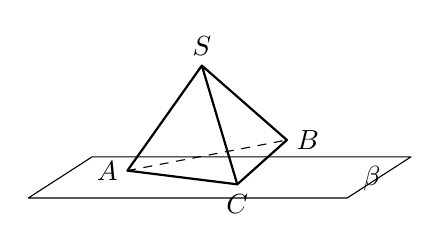
\begin{tikzpicture}[x=0.9cm,y=0.58cm,line cap=round,line join=round]
  \coordinate (P1) at (-2.4,-0.55);
  \coordinate (P2) at (2.1,-0.55);
  \coordinate (P3) at (3.0,0.35);
  \coordinate (P4) at (-1.5,0.35);
  \coordinate (A) at (-1.0,0.05);
  \coordinate (B) at (1.25,0.72);
  \coordinate (C) at (0.55,-0.25);
  \coordinate (S) at (0.05,2.35);
  \draw[thin] (P1)--(P2)--(P3)--(P4)--cycle;
  \node at (2.45,-0.12) {$\beta$};
  \draw[thick] (A)--(C)--(B);
  \draw[dashed] (A)--(B);
  \draw[thick] (S)--(A) (S)--(B) (S)--(C);
  \node[left] at (A) {$A$};
  \node[right] at (B) {$B$};
  \node[below] at (C) {$C$};
  \node[above] at (S) {$S$};
\end{tikzpicture}
\end{center}
\nopagebreak[4]
（1） 求证：$AC=BC$；

（2） 又设点 $S$ 与平面 $\beta$ 的距离为 $3$ 厘米，且 $AC\perp BC$，$AB=4$ 厘米，求线段 $SC$ 的长。

\end{question}
\begin{question}
\gktiwithlabel{29}{四}（本题满分14分）

已知复数 $z=1-2i$，其中 $i$ 是虚数单位。

（1） 求 $\dfrac2{z+i}-\overline{(z+1)}$ 的值，并把该值表示成三角形式；

\Needspace{5\baselineskip}
（2） 求适合不等式
\nopagebreak[4]
\[
\log_{0.5}\frac{|az-i|}{\sqrt{a+1}}\le\frac12
\]
的实数 $a$ 的取值范围。

\end{question}
\begin{question}
\gktiwithlabel{30}{五}（本题满分14分）

\Needspace{5\baselineskip}
设圆 $O$ 的方程为
\nopagebreak[4]
\[
x^2-2x\cos\theta+y^2+2(1+2\sin\theta)y=0,
\qquad 0\le\theta<2\pi.
\]

（1） 当 $\theta$ 变化时，求圆 $O$ 的圆心轨迹的普通方程，并画出轨迹的草图；

\Needspace{5\baselineskip}
（2） 如果又有圆 $S$：
\nopagebreak[4]
\[
x^2+y^2+2y=0,
\]
求 $\theta$ 的值，使得圆 $O$ 与圆 $S$ 的公共弦的长度取最大值（请把满足条件的 $\theta$ 的值都求出来）。

\end{question}
\end{document}
